\section{Feature Extraction}
\index{Feature Extraction}
\index{Methodology!Feature Extraction}

$Revision: 1.14 $

This section outlines some concrete implementations of feature extraction methods of the {\marf} project.
First we present you with the API and structure, followed
by the description of the methods. The class diagram of this
module set is in \xf{fig:feat}.

\begin{figure}
	\centering
	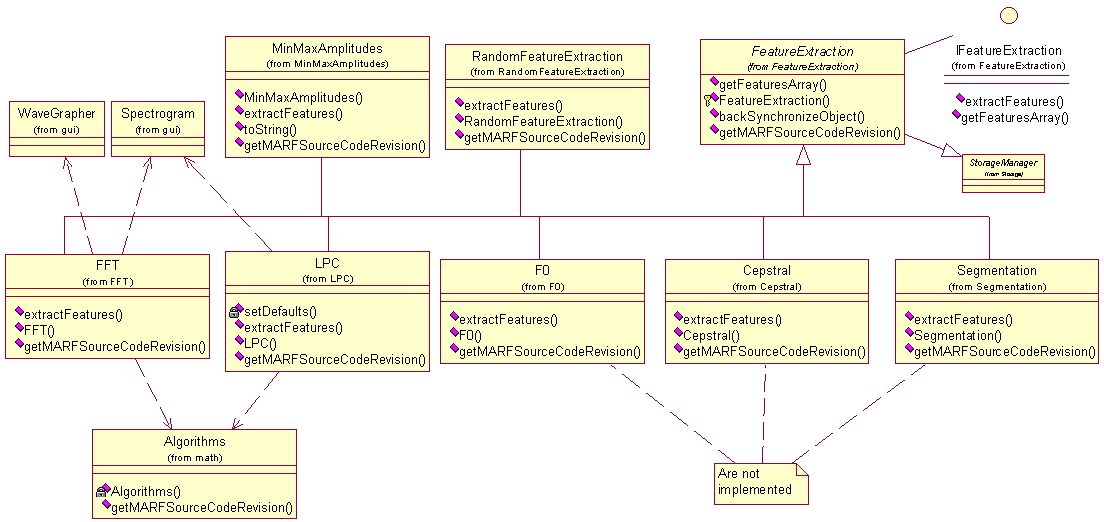
\includegraphics[angle=90,height=660pt]{../graphics/arch/feature-extraction.png}
	\caption{Feature Extraction Class Diagram}
	\label{fig:feat}
\end{figure}

\subsection{Hamming Window}
\index{Hamming Window}

$Revision: 1.13 $

\subsubsection{Implementation}
\index{Hamming Window!Implementation}

The Hamming Window implementation in {\marf} is in the
\api{marf.math.Algortithms.Hamming} class as of
version 0.3.0-devel-20050606 (a.k.a 0.3.0.2).

\subsubsection{Theory}
\index{Hamming Window!Theory}

In many DSP techniques, it is necessary to consider a smaller portion of the
entire speech sample rather than attempting to process the entire sample at
once.  The technique of cutting a sample into smaller pieces to be considered
individually is called ``windowing''.  The simplest kind of window to use is
the ``rectangle'', which is simply an unmodified cut from the larger sample.

$$
r(t) =
\left\{
{
	\begin{array}{ll}
		1 & \mbox{ for } (0 \le t \le N-1) \\
		0 & \mbox{ otherwise }
	\end{array}
}
\right.
$$

Unfortunately, rectangular windows can introduce errors, because near the edges
of the window there will potentially be a sudden drop from a high amplitude
to nothing, which can produce false ``pops'' and ``clicks'' in the analysis.

A better way to window the sample is to slowly fade out toward the edges, by
multiplying the points in the window by a ``window function''.  If we take
successive windows side by side, with the edges faded out, we will distort
our analysis because the sample has been modified by the window function.
To avoid this, it is necessary to overlap the windows so that all points in
the sample will be considered equally.  Ideally, to avoid all distortion, the
overlapped window functions should add up to a constant.  This is exactly what
the Hamming window does.  It is defined as:

$$ x = 0.54 - 0.46 \cdot \cos\left(\frac{2 \pi n}{l-1}\right) $$

\noindent
where $x$ is the new sample amplitude, $n$ is the index into the window, and $l$ is
the total length of the window.

% EOF


\subsection{Fast Fourier Transform (FFT)}\label{sect:fft}

The Fast Fourier Transform (FFT) algorithm is used both for feature extraction and as the basis for the
filter algorithm used in preprocessing.  Although a complete discussion of the
FFT algorithm is beyond the scope of this document, a short description of the
implementation will be provided here.

Essentially the FFT is an optimized version of the Discrete Fourier Transform.
It takes a window of size $2^{k}$ and returns a complex array of coefficients
for the corresponding frequency curve.  For feature extraction, only the
magnitudes of the complex values are used, while the FFT filter operates
directly on the complex results.

The implementation involves two steps: First, shuffling the input positions by a
binary reversion process, and then combining the results via a ``butterfly''
decimation in time to produce the final frequency coefficients.
The first step corresponds to breaking down the time-domain sample of size $n$
into $n$ frequency-domain samples of size 1.  The second step re-combines the $n$
samples of size 1 into 1 n-sized frequency-domain sample.

The code used in {\marf} has been translated from the C code provided in the book,
``Numeric Recipes in C'', \cite{numericalrecipes}.

\subsubsection{FFT Feature Extraction}

The frequency-domain view of a window of a time-domain sample gives us the
frequency characteristics of that window.  In feature identification, the
frequency characteristics of a voice can be considered as a list of ``features''
for that voice.  If we combine all windows of a vocal sample by
taking the average between them, we can get the average frequency
characteristics of the sample.  Subsequently, if we average the frequency
characteristics for samples from the same speaker, we are essentially finding
the center of the cluster for the speaker's samples.  Once all speakers have
their cluster centers recorded in the training set, the speaker of an
input sample should be identifiable by comparing its frequency analysis with
each cluster center by some classification method.

Since we are dealing with speech, greater accuracy should be attainable by
comparing corresponding phonemes with each other.  That is, ``th'' in ``the''
should bear greater similarity to ``th'' in ``this'' than will ``the" and ``this'' when
compared as a whole.

The only characteristic of the FFT to worry about is the window used as input.
Using a normal rectangular window can result in glitches in the frequency
analysis because a sudden cutoff of a high frequency may distort the results.
Therefore it is necessary to apply a Hamming window to the input sample, and
to overlap the windows by half.  Since the Hamming window adds up to a constant
when overlapped, no distortion is introduced.

When comparing phonemes, a window size of about 2 or 3 ms is appropriate, but
when comparing whole words, a window size of about 20 ms is more likely to be
useful.  A larger window size produces a higher resolution in the frequency
analysis.


\subsection{Linear Predictive Coding (LPC)}\label{sect:lpc}\index{LPC}

This section presents implementation of the LPC Classification module.

One method of feature extraction used in the {\marf} project was Linear
Predictive Coding (LPC) analysis. It evaluates windowed sections of
input speech waveforms and determines a set of coefficients
approximating the amplitude vs. frequency function. This approximation
aims to replicate the results of the Fast Fourier Transform yet only
store a limited amount of information: that which is most valuable to
the analysis of speech.

\subsubsection{Theory}

The LPC method is based on the formation of a spectral shaping filter,
$H(z)$, that, when applied to a input excitation source, $U(z)$, yields a
speech sample similar to the initial signal. The excitation source,
$U(z)$, is assumed to be a flat spectrum leaving all the useful
information in $H(z)$. The model of shaping filter used in most LPC
implementation is called an ``all-pole'' model, and is as follows:

$$ H(z) = \frac{G}{\left(1 - \displaystyle\sum_{k=1}^{p}(a_{k} z^{-k})\right)} $$

Where $p$ is the number of poles used. A pole is a root of the
denominator in the Laplace transform of the input-to-output
representation of the speech signal.

The coefficients $a_{k}$ are the final representation if the speech
waveform. To obtain these coefficients, the least-square
autocorrelation method was used. This method requires the use of the
autocorrelation of a signal defined as:

$$ R(k) = \displaystyle\sum_{m=k}^{n-1}(x(n) \cdot x(n-k)) $$

where $x(n)$ is the windowed input signal.

In the LPC analysis, the error in the approximation is used to derive
the algorithm. The error at time n can be expressed in the following
manner: $ e(n) = s(n) - \displaystyle\sum_{k=1}^{p}\left(a_{k} \cdot s(n-k)\right) $. Thusly,
the complete squared error of the spectral shaping filter $H(z)$ is:

$$ E = \displaystyle\sum_{n=-\infty}^{\infty}\left(x(n) - \displaystyle\sum_{k=1}^{p}(a_{k} \cdot x(n-k))\right) $$

To minimize the error, the partial derivative $\frac{{\delta}E}{{\delta}a_{k}}$ is
taken for each $k=1..p$, which yields $p$ linear equations of the form:

$$ \displaystyle\sum_{n=-\infty}^{\infty}(x(n-i) \cdot x(n)) = \displaystyle\sum_{k=1}^{p}(a_{k} \cdot \displaystyle\sum_{n=-\infty}^{\infty}(x(n-i) \cdot x(n-k)) $$

For $i=1..p$. Which, using the autocorrelation function, is:

$$ \displaystyle\sum_{k=1}^{p}(a_{k} \cdot R(i-k)) = R(i) $$

Solving these as a set of linear equations and observing that the
matrix of autocorrelation values is a Toeplitz matrix yields the
following recursive algorithm for determining the LPC coefficients:

$$ k_{m} = \frac{\left(R(m) - \displaystyle\sum_{k=1}^{m-1}\left(a_{m-1}(k)R(m-k)\right)\right)}{E_{m-1}} $$

$$ a_{m}(m) = k_{m} $$

$$ a_{m}(k) = a_{m-1}(k) - k_{m} \cdot a_{m}(m-k) \mbox{ for } 1 \le k \le m-1\mbox{,} $$

$$ E_{m} = (1 - k_{m}^2) \cdot E_{m-1} $$.

This is the algorithm implemented in the {\marf} LPC module.

\subsubsection{Usage for Feature Extraction}

The LPC coefficients were evaluated at each windowed iteration,
yielding a vector of coefficient of size $p$. These coefficients were
averaged across the whole signal to give a mean coefficient vector
representing the utterance. Thus a $p$ sized vector was used for
training and testing. The value of $p$ chosen was based on tests given
speed vs. accuracy. A $p$ value of around 20 was observed to be accurate and
computationally feasible.


\subsection{F0: The Fundamental Frequency}
\label{sect:f0}
\index{F0}
\index{Feature Extraction!F0}

$Revision: 1.6 $

[WORK ON THIS SECTION IS IN PROGRESS AS WE PROCEED WITH F0 IMPLEMENTATION IN {\marf}]

F0, the fundamental frequency, or ``pitch''.

Ian: ``The text (\cite{shaughnessy2000}) doesn't go into too much detail but gives a few techniques. Most
seem to involve another preprocessing to remove high frequencies and then
some estimation and postprocessing correction. Another, more detailed
source may be needed.''

Serguei: ``One of the prerequisites we already have: the low-pass filter that
does remove the high frequencies.''

% EOF


\subsection{Min/Max Amplitudes}
\label{sect:minmax}
\index{Min/Max Amplitudes}
\index{Feature Extraction!Min/Max Amplitudes}

$Revision: 1.4 $

\subsubsection{Description}

The Min/Max Amplitudes extraction simply involves
picking up $X$ maximums and $N$ minimums out of the
sample as features. If the length of the sample
is less than $X+N$, the difference is filled in
with the middle element of the sample.

TODO: This feature extraction does not perform very well yet
in any configuration because of the simplistic implementation:
the sample amplitudes are sorted and $N$ minimums and $X$ maximums
are picked up from both ends of the array. As the samples are
usually large, the values in each group are really close if
not identical making it hard for any of the classifiers
to properly discriminate the subjects. The future improvements
here will include attempts to pick up values in $N$ and $X$
distinct enough to be features and for the samples smaller than the $X+N$ sum,
use increments of the difference of smallest maximum and
largest minimum divided among missing elements in the middle
instead one the same value filling that space in.

% EOF


\subsection{Feature Extraction Aggregation}
\label{sect:aggregator}
\index{Feature Extraction Aggragation}
\index{Feature Extraction!Feature Extraction Aggragation}

$Revision: 1.2 $

\subsubsection{Description}

This method appeared in {\marf} as of 0.3.0.5.
This class by itself does not do any feature extraction, but
instead allows concatenation of the results of several actual feature
extractors to be combined in a single result. This should give the
classification modules more discriminatory power (e.g. when combining
the results of FFT and F0 together).
\api{FeatureExtractionAggregator} itself still implements
the \api{FeatureExtraction} API in order to be used in the main
pipeline of \api{MARF}.

The aggregator expects \api{ModuleParams} to be set to the
enumeration constants of a module to be invoked followed by that module's
enclosed instance \api{ModuleParams}. As of this implementation,
that enclosed instance of \api{ModuleParams} isn't really used, so
the {\bf main limitation} of the aggregator is that all the aggregated
feature extractors act with their default settings. This will happen until
the pipeline is re-designed a bit to include this capability.

The aggregator clones the incoming preprocessed sample for each
feature extractor and runs each module in a separate thread. A the
end, the results of each tread are collected in the same order as
specified by the initial \api{ModuleParams} and returned
as a concatenated feature vector. Some meta-information is available
if needed.

\subsubsection{Implementation}

Class: \api{marf.FeatureExtraction.FeatureExtractionAggregator}.

% EOF


\subsection{Random Feature Extraction}

By default given a window of size 256 samples, it picks
at random a number from a Gaussian distribution, and
multiplies by the incoming sample frequencies.
This all adds up and we have a feature vector at the end.
This should be the bottom line performance of all feature
extraction methods. It can also be used as a relatively fast
testing module.


% EOF
